\chapter{正弦稳态与阻抗}\label{ch:b1:sinusoidal-impedance}

转动老式收音机的调谐旋钮，在同时抵达天线的上百个电台中，
只有一个电台能够通过：线圈与可变电容器已被调谐，
恰好只有一个频率能使它们发生共振。
每面墙里嗡嗡作响的市电是 \qty{50}{Hz} 的正弦量；
用它驱动大型电动机的工厂，若其电流
滞后于\omterm{def:b1:dc-circuits:voltage}{电压}过多，就要被罚款。正弦量是\omterm{def:b1:dc-circuits:linear}{线性电路}的
“自然语言”——输出与输入形式相同，只是幅度被缩放、\omterm{def:b1:wave-propagation:signal}{相位}被平移，
并由此给出它们的代数方法：\omterm{def:b1:sinusoidal-impedance:complex}{复振幅}、
\omterm{def:b1:sinusoidal-impedance:impedance}{阻抗}、RLC 电路的共振，以及正弦电流
实际输送的功率。

\begin{omfigure}
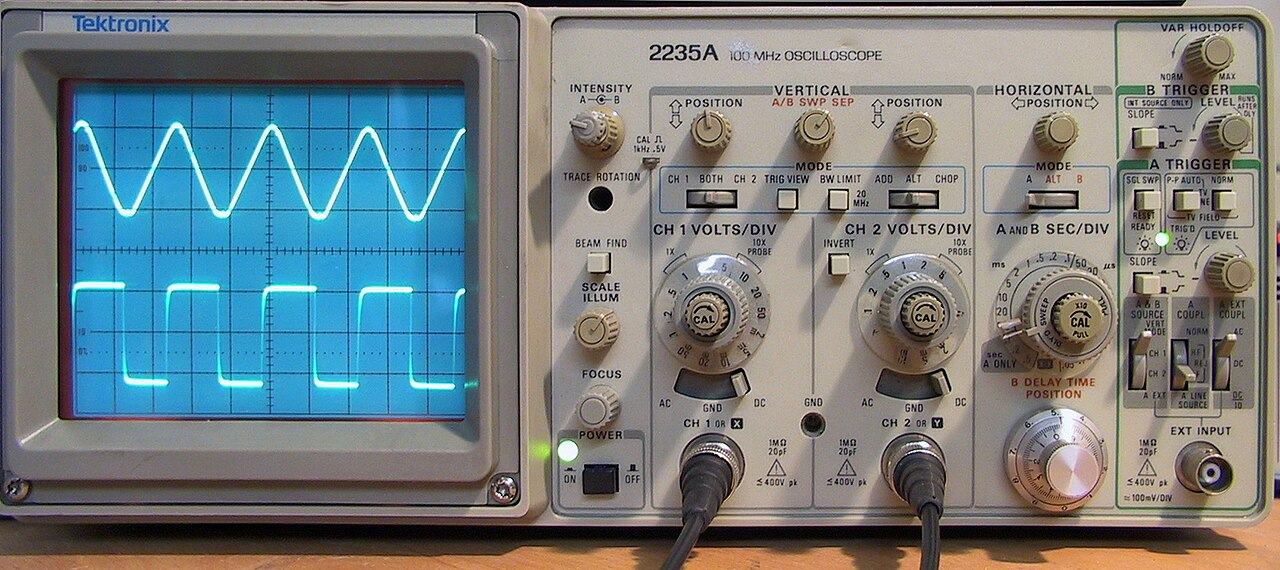
\includegraphics[width=0.60\linewidth]{images/book3/oscilloscope-sine-square.jpg}

{\small 示波器显示的一个正弦波和一个方波：正弦波是本章研究的\omterm{def:b1:wave-propagation:signal}{信号}，方波则是下一章要分解为正弦量的\omterm{def:b1:wave-propagation:signal}{信号}。}
\end{omfigure}

\section{正弦稳态}

\begin{proposition}[强迫正弦运行状态]\label{prop:b1:sinusoidal-impedance:forced}
\index{正弦稳态}\index{强迫运行状态}
在由正弦源驱动的\omterm{def:b1:dc-circuits:linear}{线性电路}中，该源的\omterm{def:b1:wave-propagation:signal}{角频率}为
$\omega$，待\omterm{def:b1:transient-regimes:firstorder}{暂态}衰减完毕后，每个电流和\omterm{def:b1:dc-circuits:voltage}{电压}都是
\omterm{def:b1:wave-propagation:signal}{角频率}同为 $\omega$ 的正弦量，各自有自己的幅值与\omterm{def:b1:wave-propagation:signal}{相位}：
$x(t) = X\cos(\omega t + \varphi)$。
\end{proposition}

\begin{proof}
电路方程是常系数线性微分方程，
其通解等于一个特解加上齐次方程的解，
齐次方程的解即
在\cref{ch:b1:transient-regimes}中的\omterm{def:b1:transient-regimes:firstorder}{暂态}，它们会衰减（每个实际电路都具有
一定电阻）。正弦特解存在，因为
对频率为 $\omega$ 的正弦量求导，所得仍是
同频率的正弦量：方程可逐项满足——
下面的复数方法将显式地构造出这一特解。
\end{proof}

\begin{definition}[复振幅]\label{def:b1:sinusoidal-impedance:complex}
\index{复振幅}\index{相量}
对于正弦量 $x(t) = X\cos(\omega t + \varphi)$，可对应一个
复\omterm{def:b1:wave-propagation:signal}{信号} $\underline{x}(t) = X\eu^{j(\omega t + \varphi)}$，使得
$x = \Rea(\underline{x})$，并称\emph{复\omterm{def:b1:wave-propagation:signal}{振幅}}
\[
\underline{X} = X\eu^{j\varphi}, \qquad \underline{x}(t) = \underline{X}\,\eu^{j\omega t},
\]
它包含幅值 $X = \abs{\underline{X}}$ 与\omterm{def:b1:wave-propagation:signal}{相位}
$\varphi = \arg\underline{X}$。这里 $j$ 表示虚单位，
$j^2 = -1$，字母 $i$ 留给电流。以长度为
$X$、与实轴夹角为 $\varphi$ 的矢量表示 $\underline{X}$ 时，
它称为\emph{相量}（菲涅耳矢量）。
\end{definition}

\begin{proposition}[复数方法的运算法则]\label{prop:b1:sinusoidal-impedance:rules}
\begin{enumerate}
  \item 线性运算与取实部可以交换次序：
        和的\omterm{def:b1:sinusoidal-impedance:complex}{复振幅}等于各\omterm{def:b1:sinusoidal-impedance:complex}{复振幅}之和。
  \item 对时间求导，\omterm{def:b1:sinusoidal-impedance:complex}{复振幅}乘以 $j\omega$；
        对时间积分则除以 $j\omega$。
  \item 基尔霍夫定律是线性的，对\omterm{def:b1:sinusoidal-impedance:complex}{复振幅}同样成立。
\end{enumerate}
\end{proposition}

\begin{proof}
$\Rea(\underline a + \underline b) = \Rea\underline a + \Rea\underline b$;
$\dd(\underline X\eu^{j\omega t})/\dd t = j\omega\underline X\eu^{j\omega t}$,
$\dd x/\dd t = \Rea(\dd\underline x/\dd t)$，因为微分是实线性的；
节点处电流之和与沿回路的\omterm{def:b1:dc-circuits:voltage}{电压}之和
都是线性的。
\end{proof}

\begin{example}[两个正弦量相加]\label{ex:b1:sinusoidal-impedance:add}
$3\cos\omega t + 4\sin\omega t$：两者的\omterm{def:b1:sinusoidal-impedance:complex}{复振幅}分别为 $3$ 和
$4\eu^{-j\pi/2} = -4j$（因为 $\sin\omega t = \cos(\omega t - \pi/2)$）；
它们之和 $3 - 4j$ 的模为 $5$，辐角为 $-0.927\ \unit{rad}$：
$5\cos(\omega t - 0.927)$。无需使用三角恒等式。
\end{example}

\section{阻抗}

\begin{definition}[阻抗、导纳]\label{def:b1:sinusoidal-impedance:impedance}
\index{阻抗}\index{导纳}\index{电抗}
对于处于\omterm{prop:b1:sinusoidal-impedance:forced}{正弦稳态}的\omterm{def:b1:dc-circuits:linear}{线性二端元件}（采用
关联参考方向），\emph{阻抗}为\omterm{def:b1:sinusoidal-impedance:complex}{复振幅}之比：
\[
\underline Z = \frac{\underline U}{\underline I} = Z\eu^{j\varphi}
\quad (\text{欧姆}),
\]
其模 $Z = U/I$ 联系两者的幅值，其辐角
$\varphi = \varphi_u - \varphi_i$ 即\omterm{def:b1:dc-circuits:voltage}{电压}超前于
电流的\omterm{def:b1:wave-propagation:signal}{相位}差。其倒数 $\underline Y = 1/\underline Z$ 称为
\emph{导纳}（单位：西门子）。$\underline Z$ 的实部称为其
电阻，虚部称为其\emph{电抗}。
\end{definition}

\begin{proposition}[R、L、C 的阻抗]\label{prop:b1:sinusoidal-impedance:rlc}
\[
\underline Z_R = R, \qquad \underline Z_L = jL\omega, \qquad
\underline Z_C = \frac{1}{jC\omega} = -\frac{j}{C\omega} .
\]
电阻使\omterm{def:b1:dc-circuits:voltage}{电压}与电流同相；线圈中的\omterm{def:b1:dc-circuits:voltage}{电压}
超前电流 $\pi/2$；电容器中的\omterm{def:b1:dc-circuits:voltage}{电压}滞后 $\pi/2$。低频时
线圈趋于导线，电容器趋于断开的电路；
高频时则相反。
\end{proposition}

\begin{proof}
$u = Ri$; $u = L\,\dd i/\dd t \to \underline U = jL\omega\,\underline I$;
$i = C\,\dd u/\dd t \to \underline I = jC\omega\,\underline U$。
其中 $1$、$j$、$-j$ 的辐角依次为 $0$、$\pi/2$、$-\pi/2$。
\end{proof}

\begin{proposition}[关联；分压与分流；定理]\label{prop:b1:sinusoidal-impedance:assoc}
串联\omterm{def:b1:sinusoidal-impedance:impedance}{阻抗}相加；并联\omterm{def:b1:sinusoidal-impedance:impedance}{导纳}相加；\omterm{def:b1:dc-circuits:voltage}{电压}与电流的分压、
分流规则，戴维南定理与诺顿定理、叠加原理，以及
\cref{ch:b1:dc-circuits} 中的米尔曼定理，
均对\omterm{def:b1:sinusoidal-impedance:complex}{复振幅}与\omterm{def:b1:sinusoidal-impedance:impedance}{阻抗}成立，只需以之代替实\omterm{def:b1:dc-circuits:voltage}{电压}、实电流
与电阻。
\end{proposition}

\begin{proof}
\cref{ch:b1:dc-circuits} 中的每个证明都只用到基尔霍夫定律
与 $u = Ri$ 的线性性，二者在复数形式下均成立。
\end{proof}

\begin{example}[RC 分压器]\label{ex:b1:sinusoidal-impedance:rcdivider}
\omterm{def:b1:dc-circuits:resistor}{电阻器} $R$ 与电容器 $C$ 串联后接在 $\underline E$ 两端，
输出取自 $C$ 两端：$\underline U_C = \underline E\,\dfrac{1/jC\omega}
{R + 1/jC\omega} = \dfrac{\underline E}{1 + jRC\omega}$。\omterm{def:b1:wave-propagation:signal}{振幅}
$E/\sqrt{1 + (RC\omega)^2}$，\omterm{def:b1:wave-propagation:signal}{相位} $-\arctan(RC\omega)$：低频时完全透射，
幅值为 $1/\sqrt2$、\omterm{def:b1:wave-propagation:signal}{相位}为 $-45^\circ$ 的点位于
$\omega = 1/RC$ 处，此后按 $1/\omega$ 下降——这是一个低通滤波器，
即 \cref{ch:b1:filters-transfer-functions} 的研究对象。
\end{example}

\section{串联 RLC 电路：共振}

\begin{theorem}[电流共振]\label{thm:b1:sinusoidal-impedance:resonance}
\index{共振}\index{共振!电流}\index{带宽}
\omterm{def:b1:dc-circuits:resistor}{电阻器} $R$、线圈 $L$ 与电容器 $C$ 串联后接在
$e(t) = E\cos\omega t$ 两端，电流的\omterm{def:b1:sinusoidal-impedance:complex}{复振幅}为
\[
\underline I = \frac{E}{R + j\left(L\omega - \dfrac{1}{C\omega}\right)},
\qquad
I = \frac{E}{\sqrt{R^2 + \left(L\omega - \dfrac{1}{C\omega}\right)^2}},
\qquad
\varphi_i = -\arctan\frac{L\omega - 1/C\omega}{R} .
\]
\omterm{def:b1:wave-propagation:signal}{振幅}最大，$I_{\max} = E/R$，此时电流与\omterm{def:b1:dc-circuits:voltage}{电压}同相，
即在\emph{共振}频率 $\omega_0 = 1/\sqrt{LC}$ 处取得。记
$Q = L\omega_0/R = 1/(RC\omega_0)$，$x = \omega/\omega_0$，则
\[
\frac{I}{I_{\max}} = \frac{1}{\sqrt{1 + Q^2\left(x - \dfrac1x\right)^2}} ,
\]
而\emph{带宽}——即 $\omega$ 的取值区间，
其中 $I \geq I_{\max}/\sqrt2$ ——为
\[
\Delta\omega = \omega_2 - \omega_1 = \frac{\omega_0}{Q} = \frac{R}{L} .
\]
\end{theorem}

\begin{proof}
串联\omterm{def:b1:sinusoidal-impedance:impedance}{阻抗}相加：$\underline Z = R + jL\omega + 1/jC\omega$，且
$\underline I = \underline E/\underline Z$。电流的模在
\omterm{def:b1:sinusoidal-impedance:impedance}{电抗} $L\omega - 1/C\omega$ 为零时最大，即在 $\omega_0$ 处。
将 $L\omega - 1/C\omega = L\omega_0(x - 1/x)$ 因式分解，再除以 $R$：
$L\omega_0/R = Q$。带宽边界处 $Q(x - 1/x) = \pm 1$，即
$x^2 \mp x/Q - 1 = 0$，其正根为 $x_{1,2} = \mp\frac{1}{2Q}
+ \sqrt{1 + \frac{1}{4Q^2}}$；二者之差为 $1/Q$。
\end{proof}

\begin{omfigure}
\begin{tikzpicture}
\begin{axis}[omaxis, width=7.6cm, height=5.4cm, xlabel={$\omega/\omega_0$}, ylabel={$I/I_{\max}$},
    xmin=0, xmax=2.1, ymin=0, ymax=1.45, xtick={0.5,1,1.5,2}, ytick={0.5,0.707,1},
    yticklabels={$0.5$,$\frac{1}{\sqrt2}$,$1$},
    legend style={at={(0.97,0.97)}, anchor=north east, font=\footnotesize, draw=none, fill=none}]
  \addplot[omProp, thick, domain=0.05:2.1, samples=300] {1/sqrt(1 + (1*(x - 1/x))^2)};
  \addlegendentry{$Q = 1$}
  \addplot[omDef, thick, domain=0.05:2.1, samples=300] {1/sqrt(1 + (3*(x - 1/x))^2)};
  \addlegendentry{$Q = 3$}
  \addplot[omThm, thick, domain=0.05:2.1, samples=500] {1/sqrt(1 + (10*(x - 1/x))^2)};
  \addlegendentry{$Q = 10$}
  \draw[dashed, omExo] (axis cs:0,0.707) -- (axis cs:2.1,0.707);
\end{axis}
\end{tikzpicture}\qquad
\begin{tikzpicture}
\begin{axis}[omaxis, width=7.0cm, height=5.4cm, xlabel={$\omega/\omega_0$}, ylabel={$\varphi_i$},
    xmin=0, xmax=2.1, ymin=-1.8, ymax=1.8, xtick={0.5,1,1.5,2}, ytick={-1.5708,0,1.5708},
    yticklabels={$-\frac{\pi}{2}$,$0$,$\frac{\pi}{2}$}]
  \addplot[omProp, thick, domain=0.05:2.1, samples=300] {-rad(atan(1*(x - 1/x)))};
  \addplot[omDef, thick, domain=0.05:2.1, samples=300] {-rad(atan(3*(x - 1/x)))};
  \addplot[omThm, thick, domain=0.05:2.1, samples=500] {-rad(atan(10*(x - 1/x)))};
\end{axis}
\end{tikzpicture}

{\small 串联 RLC 电路：电流的\omterm{def:b1:wave-propagation:signal}{振幅}（左）及其相对于电源的\omterm{def:b1:wave-propagation:signal}{相位}（右），
随 $\omega/\omega_0$ 变化，
取 $Q = 1, 3, 10$。峰值随 $Q$ 增大而变窄（$\Delta\omega =
\omega_0/Q$）；低于共振时电路呈容性（电流超前），
高于共振时则呈感性（电流滞后）。}
\end{omfigure}

\begin{omfigure}
\begin{tikzpicture}[font=\small, x=1cm, y=1cm, >=Stealth]
  % phasors for RLC at omega above resonance: UR along I, UL +90, UC -90
  \draw[->, thick, omExo] (0,0) -- (2.6,0) node[right] {$\underline I$};
  \draw[->, very thick, omProp] (0,0) -- (1.6,0) node[midway, below] {$\underline U_R = R\underline I$};
  \draw[->, very thick, omDef] (1.6,0) -- (1.6,2.4) node[left, pos=0.8] {$\underline U_L = jL\omega\underline I$};
  \draw[->, very thick, omDef!60] (1.78,2.4) -- (1.78,1.1) node[right, midway] {$\underline U_C = \underline I/jC\omega$};
  \draw[->, very thick, omThm] (0,0) -- (1.6,1.1) node[midway, above left, xshift=-1pt] {$\underline E$};
  \draw (0.6,0) arc (0:34.5:0.6); \node at (0.85,0.2) {$\varphi$};
\end{tikzpicture}

{\small 串联 RLC 电路高于共振频率时的\omterm{def:b1:sinusoidal-impedance:complex}{相量}图：$\underline U_R$
沿 $\underline I$ 方向，$\underline U_L$ 超前四分之一周，$\underline U_C$
滞后四分之一周；它们的和 $\underline E$ 较电流
超前 $\varphi$。共振时 $\underline U_L$ 与 $\underline U_C$ 相互抵消，
从而 $\underline E = \underline U_R$。}
\end{omfigure}

\begin{proposition}[电压放大率]\label{prop:b1:sinusoidal-impedance:overvoltage}
\index{共振!电压}\index{过电压}
共振时，线圈与电容器两端的\omterm{def:b1:dc-circuits:voltage}{电压}\omterm{def:b1:wave-propagation:signal}{振幅}相同，
均为 $QE$，\omterm{def:b1:wave-propagation:signal}{相位}相反；当 $Q \gg 1$ 时，电容器
两端的\omterm{def:b1:dc-circuits:voltage}{电压}是电源\omterm{def:b1:dc-circuits:voltage}{电压}的 $Q$ 倍。\omterm{def:b1:wave-propagation:signal}{振幅}
$U_C(\omega)$ 本身在 $Q > 1/\sqrt2$ 时取峰值，峰值位置为 $\omega_r =
\omega_0\sqrt{1 - 1/2Q^2}$，略低于 $\omega_0$，此时
$U_{C,\max} = QE/\sqrt{1 - 1/4Q^2}$。
\end{proposition}

\begin{proof}
在 $\omega_0$ 处，$\underline U_C = \underline I/jC\omega_0 = -jQE$，
$\underline U_L = jL\omega_0\underline I = jQE$（因 $I = E/R$）。
一般地，$U_C = I/C\omega = E/\sqrt{(1 - x^2)^2 + x^2/Q^2}$（
分子与分母同乘 $1/C\omega_0$）；分母的平方
为 $(1 - x^2)^2 + x^2/Q^2$，它是关于 $x^2$ 的二次式，在 $x^2 =
1 - 1/2Q^2$ 时取最小值（须该值为正），最小值为 $1/Q^2 - 1/4Q^4$。
\end{proof}

\begin{example}[调谐收音机]\label{ex:b1:sinusoidal-impedance:radio}
一只线圈 $L = \qty{200}{\micro H}$ 与一只可变电容器：$C =
\qty{127}{pF}$ 调谐于 $f_0 = \qty{1.00}{MHz}$。线圈导线的
电阻 $R = \qty{12.6}{\ohm}$，$L\omega_0 = \qty{1257}{\ohm}$，且
$Q = 100$：带宽 $\Delta f = f_0/Q = \qty{10}{kHz}$——
即 AM 频道的宽度——而远处发射机感应出的 \qty{10}{\micro V} \omterm{def:b1:dc-circuits:voltage}{电压}
在电容器两端变为 $QE = \qty{1}{mV}$，无需
额外放大。周末问题要求搭建这一接收机。
\end{example}

\begin{remark}[再论 $Q$]\label{rem:b1:sinusoidal-impedance:Q}
本章的 $Q$ 即\cref{ch:b1:transient-regimes}中的 $Q$：
受激后振荡约 $Q$ 次的电路，
也正是受驱动时在宽为 $\omega_0/Q$ 的频带上共振的那个电路。两者
都表示同一个比值：$2\pi$ 倍的储存能量与每周期耗散能量之比
（见\cref{exo:b1:sinusoidal-impedance:12}）。尖锐的共振与持久的振铃
是同一种性质，慢响应也是
如此：带宽为 $\Delta\omega$ 的滤波器
需要约 $1/\Delta\omega$ 量级的时间才能稳定。
\end{remark}

\section{正弦稳态下的功率}

\begin{definition}[有效值]\label{def:b1:sinusoidal-impedance:rms}
\index{有效值}\index{有效值}
周期\omterm{def:b1:wave-propagation:signal}{信号}的\emph{方均根值}（rms，亦称有效值）
$x(t)$ 记为 $X_{\mathrm{rms}} = \sqrt{\langle x^2\rangle}$，即
$x^2$ 在一个周期内的时间平均值的平方根。对于
\omterm{def:b1:wave-propagation:signal}{振幅}为 $X$ 的正弦量，$X_{\mathrm{rms}} = X/\sqrt2$。市电的 \qty{230}{V}
为有效值，其\omterm{def:b1:wave-propagation:signal}{振幅}为 \qty{325}{V}。
\end{definition}

\begin{theorem}[平均功率]\label{thm:b1:sinusoidal-impedance:power}
\index{平均功率}\index{功率因数}\index{无功功率}
一个二端网络，其 $u = U\cos\omega t$，$i = I\cos(\omega t - \varphi)$
（\omterm{thm:b1:dc-circuits:kirchhoff}{受电器约定}）接收瞬时功率 $p = ui$，其
平均值为
\[
P = \tfrac12\,UI\cos\varphi = U_{\mathrm{rms}}I_{\mathrm{rms}}\cos\varphi
= \tfrac12\Rea\!\big(\underline U\,\underline I^{\,*}\big) = \tfrac12\Rea(\underline Z)\,I^2,
\]
其中 $\cos\varphi$ 称为\emph{\omterm{thm:b1:sinusoidal-impedance:power}{功率因数}}。\omterm{def:b1:dc-circuits:resistor}{电阻器}接收的功率为
$\tfrac12 RI^2 = RI_{\mathrm{rms}}^2$；理想线圈或电容器
（$\varphi = \pm\pi/2$）不接收\omterm{thm:b1:sinusoidal-impedance:power}{平均功率}——它在半个周期内储存能量，
在另外半个周期内将其释放。
\end{theorem}

\begin{proof}
$p = UI\cos\omega t\cos(\omega t - \varphi) = \tfrac12 UI[\cos\varphi +
\cos(2\omega t - \varphi)]$；第二项的时间平均为零。取
$\underline U = U$，$\underline I = I\eu^{-j\varphi}$，
则 $\underline U\,\underline I^* = UI\eu^{j\varphi}$，其实部为
$UI\cos\varphi$；又由 $\underline U = \underline Z\,\underline I$ 得
$\underline U\,\underline I^* = \underline Z I^2$。
\end{proof}

\begin{omfigure}
\begin{tikzpicture}
\begin{axis}[omaxis, axis x line=bottom, width=11.5cm, height=5cm, xlabel={$t/T$}, ylabel={$p$},
    xmin=0, xmax=2, ymin=-0.5, ymax=1.15, xtick={0.5,1,1.5,2}, ytick={0,0.5,1},
    yticklabels={$0$,$P$,$UI$}]
  \addplot[omDef, thick, domain=0:2, samples=300] {cos(deg(2*pi*x))*cos(deg(2*pi*x) - 60)};
  \addplot[omThm, thick, dashed, domain=0:2, samples=2] {0.25};
  \addplot[omExo, dashed, domain=0:2, samples=2] {0};
  \node[omDef, font=\footnotesize] at (axis cs:1.62,0.95) {$p(t) = ui$, $\varphi = 60^\circ$};
  \node[omThm, font=\footnotesize] at (axis cs:0.5,0.95) {平均 $P = \tfrac12 UI\cos\varphi$（虚线）};
\end{axis}
\end{tikzpicture}

{\small 二端网络接收的瞬时功率，电流与\omterm{def:b1:dc-circuits:voltage}{电压}之间有 $60^\circ$ 的\omterm{def:b1:wave-propagation:signal}{相位}
滞后：功率以 $2\omega$ 变化，有时降至零以下（能量回送给
电源），平均值为 $\tfrac12 UI\cos\varphi$，
——此处为同相时的一半。}
\end{omfigure}

\begin{example}[功率因数校正]\label{ex:b1:sinusoidal-impedance:pf}
一台车间电动机接在 \qty{230}{V}（\omterm{def:b1:sinusoidal-impedance:rms}{有效值}）电源上，吸收功率 \qty{2.0}{kW}，
\omterm{thm:b1:sinusoidal-impedance:power}{功率因数} $\cos\varphi = 0.70$（感性）：$I_{\mathrm{rms}} = 2000/(230 \times
0.70) = \qty{12.4}{A}$，而\omterm{thm:b1:sinusoidal-impedance:power}{功率因数}为
$1$ 时仅需 \qty{8.7}{A}：多出的电流白白使供电电缆发热，
这正是罚款的缘由。并联电容器在本地提供线圈四分之一周期内的
能量往返：\emph{\omterm{thm:b1:sinusoidal-impedance:power}{无功功率}} $P\tan\varphi =
\qty{2.0}{kvar}$，所需电容为 $C = P\tan\varphi/(\omega U_{\mathrm{rms}}^2)
\approx \qty{120}{\micro F}$（\qty{50}{Hz} 下），线路电流降至
\qty{8.7}{A}。
\end{example}

\section{练习}

\begin{exercise}[$\star$]\label{exo:b1:sinusoidal-impedance:1}
求 $u = 5\cos(\omega t + \pi/3)$（V）的\omterm{def:b1:sinusoidal-impedance:complex}{复振幅}，
分别用极坐标形式和直角坐标形式表示。利用\omterm{def:b1:sinusoidal-impedance:complex}{复振幅}，将 $3\cos\omega t
+ 4\sin\omega t$ 写成单一的余弦形式。
\end{exercise}

\begin{exercise}[$\star$]\label{exo:b1:sinusoidal-impedance:2}
计算 $R = \qty{100}{\ohm}$、$L = \qty{0.10}{H}$ 和
$C = \qty{10}{\micro F}$ 在 \qty{50}{Hz} 与 \qty{1.0}{kHz} 下的\omterm{def:b1:sinusoidal-impedance:impedance}{阻抗}。
并给出 $R$ 与 $L$ 串联后\omterm{def:b1:sinusoidal-impedance:impedance}{阻抗}的模与\omterm{def:b1:wave-propagation:signal}{相位}，
设频率为 \qty{50}{Hz}。
\end{exercise}

\begin{exercise}[$\star$]\label{exo:b1:sinusoidal-impedance:3}
电网\omterm{def:b1:dc-circuits:voltage}{电压}为\omterm{def:b1:sinusoidal-impedance:rms}{有效值} \qty{230}{V}，其\omterm{def:b1:wave-propagation:signal}{振幅}是多少？一台 \qty{2.0}{kW} 的电热器，
求其电流的\omterm{def:b1:sinusoidal-impedance:rms}{有效值}与峰值。证明电阻中的\omterm{thm:b1:sinusoidal-impedance:power}{平均功率}为
$RI_{\mathrm{rms}}^2$。
\end{exercise}

\begin{exercise}[$\star$]\label{exo:b1:sinusoidal-impedance:4}
串联 RLC 电路：$L = \qty{10}{mH}$，$C = \qty{100}{nF}$，$R = \qty{100}{\ohm}$，
$E = \qty{1.0}{V}$。求 $f_0$、$Q$、以赫兹为单位的带宽以及
共振时的电流\omterm{def:b1:wave-propagation:signal}{振幅}。
\end{exercise}

\begin{exercise}[$\star\star$]\label{exo:b1:sinusoidal-impedance:5}
RC 分压电路，输出取自 $C$：$R = \qty{1.0}{k\ohm}$，$C = \qty{159}{nF}$。
在何频率下输出为输入的 $1/\sqrt2$？求
\qty{1.0}{kHz} 与 \qty{10}{kHz} 下的输出\omterm{def:b1:wave-propagation:signal}{振幅}比与\omterm{def:b1:wave-propagation:signal}{相位}。
\end{exercise}

\begin{exercise}[$\star\star$]\label{exo:b1:sinusoidal-impedance:6}
在某一频率下，串联 RLC 电路中 $R = \qty{100}{\ohm}$，$L\omega =
\qty{250}{\ohm}$，$1/C\omega = \qty{100}{\ohm}$，$E = \qty{1.0}{V}$。
计算 $\underline Z$、电流\omterm{def:b1:wave-propagation:signal}{振幅}与\omterm{def:b1:wave-propagation:signal}{相位}以及三个
\omterm{def:b1:dc-circuits:voltage}{电压}\omterm{def:b1:wave-propagation:signal}{振幅}；画出\omterm{def:b1:sinusoidal-impedance:complex}{相量}图。电路处于共振点上方还是
下方？
\end{exercise}

\begin{exercise}[$\star\star$]\label{exo:b1:sinusoidal-impedance:7}
收音机：$L = \qty{200}{\micro H}$，$C$ 可在 \qty{50}{} 至
\qty{500}{pF} 之间\omterm{def:b1:optical-instruments:eye}{调节}。求频率范围，以及 \qty{1.00}{MHz} 时的电容，
并在 $Q = 100$ 时求带宽，以及
相距 \qty{9}{kHz} 的电台的衰减（\omterm{def:b1:wave-propagation:signal}{振幅}比）。天线电动势为
\qty{10}{\micro V}：共振时 $C$ 两端的\omterm{def:b1:dc-circuits:voltage}{电压}是多少？
\end{exercise}

\begin{exercise}[$\star\star$]\label{exo:b1:sinusoidal-impedance:8}
推导串联 RLC 电路的两个半功率频率，并证明
它们之差为 $\omega_0/Q$，之积为 $\omega_0^2$。
\end{exercise}

\begin{exercise}[$\star\star$]\label{exo:b1:sinusoidal-impedance:9}
一台电动机接在 \qty{230}{V} \omterm{def:b1:sinusoidal-impedance:rms}{有效值}、\qty{50}{Hz} 的电源上，吸收功率 \qty{2.0}{kW}，
$\cos\varphi = 0.70$。计算电流\omterm{def:b1:sinusoidal-impedance:rms}{有效值}、\omterm{thm:b1:sinusoidal-impedance:power}{无功功率}、
为使\omterm{thm:b1:sinusoidal-impedance:power}{功率因数}达到 $1$ 而并联的电容，以及
新的电流。供电线路电阻为 \qty{0.50}{\ohm}，求并联前
后的焦耳损耗。
\end{exercise}

\begin{exercise}[$\star\star\star$]\label{exo:b1:sinusoidal-impedance:10}
由\omterm{def:b1:dc-circuits:sources}{电流源}供电的并联 RLC 电路：写出\omterm{def:b1:sinusoidal-impedance:impedance}{导纳}，证明
\omterm{def:b1:dc-circuits:voltage}{电压}在 $\omega_0 = 1/\sqrt{LC}$ 处最大，且此时等于 $RI$，
并证明带宽为 $\Delta\omega = 1/RC$，即 $Q =
R\sqrt{C/L}$。数值：$R = \qty{10}{k\ohm}$，$L = \qty{1.0}{mH}$，
$C = \qty{1.0}{nF}$。
\end{exercise}

\begin{exercise}[$\star\star\star$]\label{exo:b1:sinusoidal-impedance:11}
证明串联 RLC 电路中电容器\omterm{def:b1:dc-circuits:voltage}{电压}为 $U_C = E/\sqrt{(1 -
x^2)^2 + x^2/Q^2}$，并证明其在 $x_r = \sqrt{1 - 1/2Q^2}$ 处取峰值的条件是
$Q > 1/\sqrt2$，求 $x_r$ 与 $U_{C,\max}/E$，取 $Q = 3.16$。
$Q < 1/\sqrt2$ 时情况如何？
\end{exercise}

\begin{exercise}[$\star\star\star$]\label{exo:b1:sinusoidal-impedance:12}
在串联 RLC 电路共振时，证明总储能
$\tfrac12 Li^2 + \tfrac12 Cu_C^2$ 为常量，且等于 $\tfrac12 LI^2$，
求每个周期内 $R$ 中耗散的能量，并证明
$2\pi\,(\text{储能})/(\text{每周期耗散能量}) = Q$。
\end{exercise}

\begin{omfigure}

\includegraphics[width=0.55\linewidth]{images/book3/ai/b3-08-vintage-radio-tuning.jpg}

{\small 调谐电子管收音机：转动旋钮改变电容器，电容器决定 $LC$ 电路的共振频率，频率相符的电台即为所收听的电台——即周末问题。}
\end{omfigure}

\section{问题：共振收音接收机}

\begin{problem}[{周末问题——线圈、可变电容器与天线：
串联共振如何在一百个电台中挑出一个，
将其微弱信号放大一百倍，
以及为何选择性不能被任意提高}]
\label{pb:b1:sinusoidal-impedance:1}
天线可建模为理想正弦电动势 $e(t) = E\cos\omega t$，
与电感 $L = \qty{200}{\micro H}$ 的线圈串联，线圈导线的电阻为
$R = \qty{12.6}{\ohm}$，并与可变电容器 $C$ 串联。接收机
读取 $C$ 两端的\omterm{def:b1:dc-circuits:voltage}{电压}。后文（第四部分）中将计入天线自身的
电阻 $R_a = \qty{50}{\ohm}$。

\medskip
\noindent\textbf{第一部分——共振电流。}
\begin{enumerate}
  \item 写出串联电路的复\omterm{def:b1:sinusoidal-impedance:impedance}{阻抗}。
  \item 求电流的\omterm{def:b1:sinusoidal-impedance:complex}{复振幅}，再求其\omterm{def:b1:wave-propagation:signal}{振幅}
        $I(\omega)$ 及其\omterm{def:b1:wave-propagation:signal}{相位} $\varphi_i(\omega)$（相对于 $e$）。
  \item 证明 $I$ 在 $\omega_0 = 1/\sqrt{LC}$ 处取最大值；求
        $I_{\max}$ 及此时的\omterm{def:b1:wave-propagation:signal}{相位}。
  \item 何种电容可使 $f_0 = \qty{1.000}{MHz}$ 调谐？求
        $L\omega_0$。
  \item 定义 $Q = L\omega_0/R$，并求其值。
  \item 证明 $I/I_{\max} = 1/\sqrt{1 + Q^2(x - 1/x)^2}$，其中
        $x = \omega/\omega_0$。
  \item 说明 $\varphi_i$ 在共振频率以下与以上的符号，并
        解释其呈容性还是感性。
\end{enumerate}

\medskip
\noindent\textbf{第二部分——选择性。}
\begin{enumerate}[resume]
  \item 写出确定两个频率的条件，两频率处满足
        $I = I_{\max}/\sqrt2$。
  \item 解之，并证明 $\Delta\omega = \omega_2 - \omega_1 =
        \omega_0/Q$。
  \item 求该接收机的带宽 $\Delta f$。
  \item 第二个电台发射频率为 \qty{1.010}{MHz}，第三个为
        \qty{1.020}{MHz}：分别求其\omterm{def:b1:wave-propagation:signal}{振幅}比 $I/I_{\max}$，
        以及对应的功率比（以分贝表示）。
  \item 调幅电台的间隔为 \qty{9}{} 至 \qty{10}{kHz}。该接收机的
        选择性是否足够？如何改进？
  \item 电容器可在 \qty{50}{} 与 \qty{500}{pF} 之间\omterm{def:b1:optical-instruments:eye}{调节}：
        该接收机能覆盖哪一频段？
\end{enumerate}

\medskip
\noindent\textbf{第三部分——\omterm{def:b1:dc-circuits:voltage}{电压}放大。}
\begin{enumerate}[resume]
  \item 写出电容器\omterm{def:b1:dc-circuits:voltage}{电压}的\omterm{def:b1:sinusoidal-impedance:complex}{复振幅}，并证明
        在共振时其\omterm{def:b1:wave-propagation:signal}{振幅}为 $QE$。
  \item 天线电动势为 $E = \qty{10}{\micro V}$：计算 $I_{\max}$
        及共振时的电容器\omterm{def:b1:dc-circuits:voltage}{电压}，并加以评论。
  \item 证明在共振时线圈\omterm{def:b1:dc-circuits:voltage}{电压}与电容器\omterm{def:b1:dc-circuits:voltage}{电压}的\omterm{def:b1:wave-propagation:signal}{振幅}相同，
        且两者反相，
        源“感受到”的是什么？
  \item 计算共振时电路中储存的能量，以及每个周期耗散的能量；
        验证两者之比
        乘以 $2\pi$ 等于 $Q$。
  \item 由\cref{ch:b1:transient-regimes}可知，该电路的\omterm{def:b1:transient-regimes:firstorder}{时间常数}是多少？
        即 $\tau = 2Q/\omega_0$。为什么很高的 $Q$ 最终会使语音和音乐失真
        （AM 的音频带宽约为
        \qty{5}{kHz}）？
  \item 若线圈导线的电阻加倍（导线变细），
        $Q$、带宽和电容器\omterm{def:b1:dc-circuits:voltage}{电压}将如何变化？
\end{enumerate}

\medskip
\noindent\textbf{第四部分——天线的电阻与功率。}
\begin{enumerate}[resume]
  \item 将 $R_a = \qty{50}{\ohm}$ 与电路串联，重新计算 $Q$、
        带宽和电容器\omterm{def:b1:dc-circuits:voltage}{电压}，设 $E = \qty{10}{\micro V}$。
        并作出结论。
  \item 计算共振时天线电动势提供的\omterm{thm:b1:sinusoidal-impedance:power}{平均功率}，
        以及在 $R_a$ 上耗散的比例。
  \item 最大功率定理要求负载电阻等于
        $R_a$：为什么这一目标与选择性相矛盾？
  \item 实际接收机将天线接到线圈上的一个抽头，或
        通过一个小的耦合电容器相连，定性说明
        这样做的作用。
  \item 利用 $P = \tfrac12 UI\cos\varphi$，计算
        两个半功率频率处的\omterm{thm:b1:sinusoidal-impedance:power}{功率因数}，
        并说明“半功率”这一名称的由来。
  \item 总结设计：$Q$ 带来什么、付出什么代价，以及
        对于 \qty{1}{MHz} 接收机、\qty{10}{kHz} 信道所选取的
        数值。
\end{enumerate}
\end{problem}
